\section{Simulation Analysis}
\label{sec:simulation}
In this section we will describe the steps needed to simulate this circuit using the software Ngspice. Essentially, we only need to perform transient analysis.

The following steps in the simulations were conducted: 
\begin{itemize}
	\item describing the circuit architecture in the spice script;
	\item simulating the AC/DC converter for 10 periods (200 ms, given the source frequency of 50 Hz); given the initial transient period, corresponding to the charge/discharge of the Capacitors up to operating point conditions, we considered a time period betwenn 1400ms and 1600ms, to avoid having our average and ripple values contaminated by this transient initial period, beginning at t=0ms.
	\item measuring the output voltage ripple using Ngpice’s min and
max functions: ripple($v_O$) = max($v_O$) - min($v_O$)
	\item plotting the voltages at the output of the Envelope Detector
and Voltage Regulator circuits
	\item plotting ($v_O$ – 12) (output AC component + DC deviation)
	\item recursively automating the parameter generation data with a different octave script, so as to only alter the parameters in one file and simultaneously run the simulation and the the theoretcial analysis for comparison
	\item automate the result evaluation process, in order to automatically generate the merit, given the parameters used (relating to cost) as input and the simulation results.
	\item trying to optimize the the parameters for a maximum merit. This was done by choosing values for the envelope detector (a quick analysis suggested the ideal combination would have equal numerical values for the capacitance and for the resistor in this segment of the circuit), in order to minimize ripple and cost, followed by fine-tuning the output voltage to 12V by tweaking the parameters n and Voltage Regulator resistor. Multiple iterations of this process were carried out before a "final configuration" was chosen.
	

\end{itemize}

The only significant change implemented regarding the architecture for a converter studied in class (using the full wave rectifier, which seemed, off the bat, to be the best choice), was substituting the series of diodes in the regulator for a parallel of two equal series of 20 diodes, which offered a slight advantage, as this proved to be an inexpensive way to reduce by half the equivalent incremental resistance of the regulator's diodes, and thus minimize the ripple even more. The results of the simulation (left) are repeated here, compared with the corresponding theoretical simulations.
 
\hfill
 \parbox{1\linewidth}{
  \centering
  \begin{tabular}{|l|l|l|r|}
    %\hline    
    {\bf Parameter} & {\bf Simulation} & {\bf Theoretical } & {\bf Units }\\ \hline
    Zi & 766.402 & 640.49 & Ohm\\ \hline
Zo & 4.49605 & 2.9364 & Ohm\\ \hline
Cost & 8116 & Cost & MU\\ \hline
uco & 3106933.000 & 2123123123123.000 & Hz\\ \hline
lco & 7.924 & 2123123123123.000 & Hz\\ \hline
Bandwidth & 3106925.076 & 2123123123123.000 & Hz\\ \hline
Gainv(out) & 56.041 & -107.220 & [adimensional]\\ \hline
MERIT & 2707.5316 & -104.2260 & gold medals\\ \hline

  \end{tabular}
  \label{tab:results}
    %\caption{Side-by-side comparison of the circuit parameters (resistors, capacitors, etc) and the corresponding results (ripple, average, merit)}
  }


  
%ponto 1
\subsection{Output of the Envelope Detector (acting on the output of the full-wave rectifier)}

\par
\begin{figure}[H] \centering
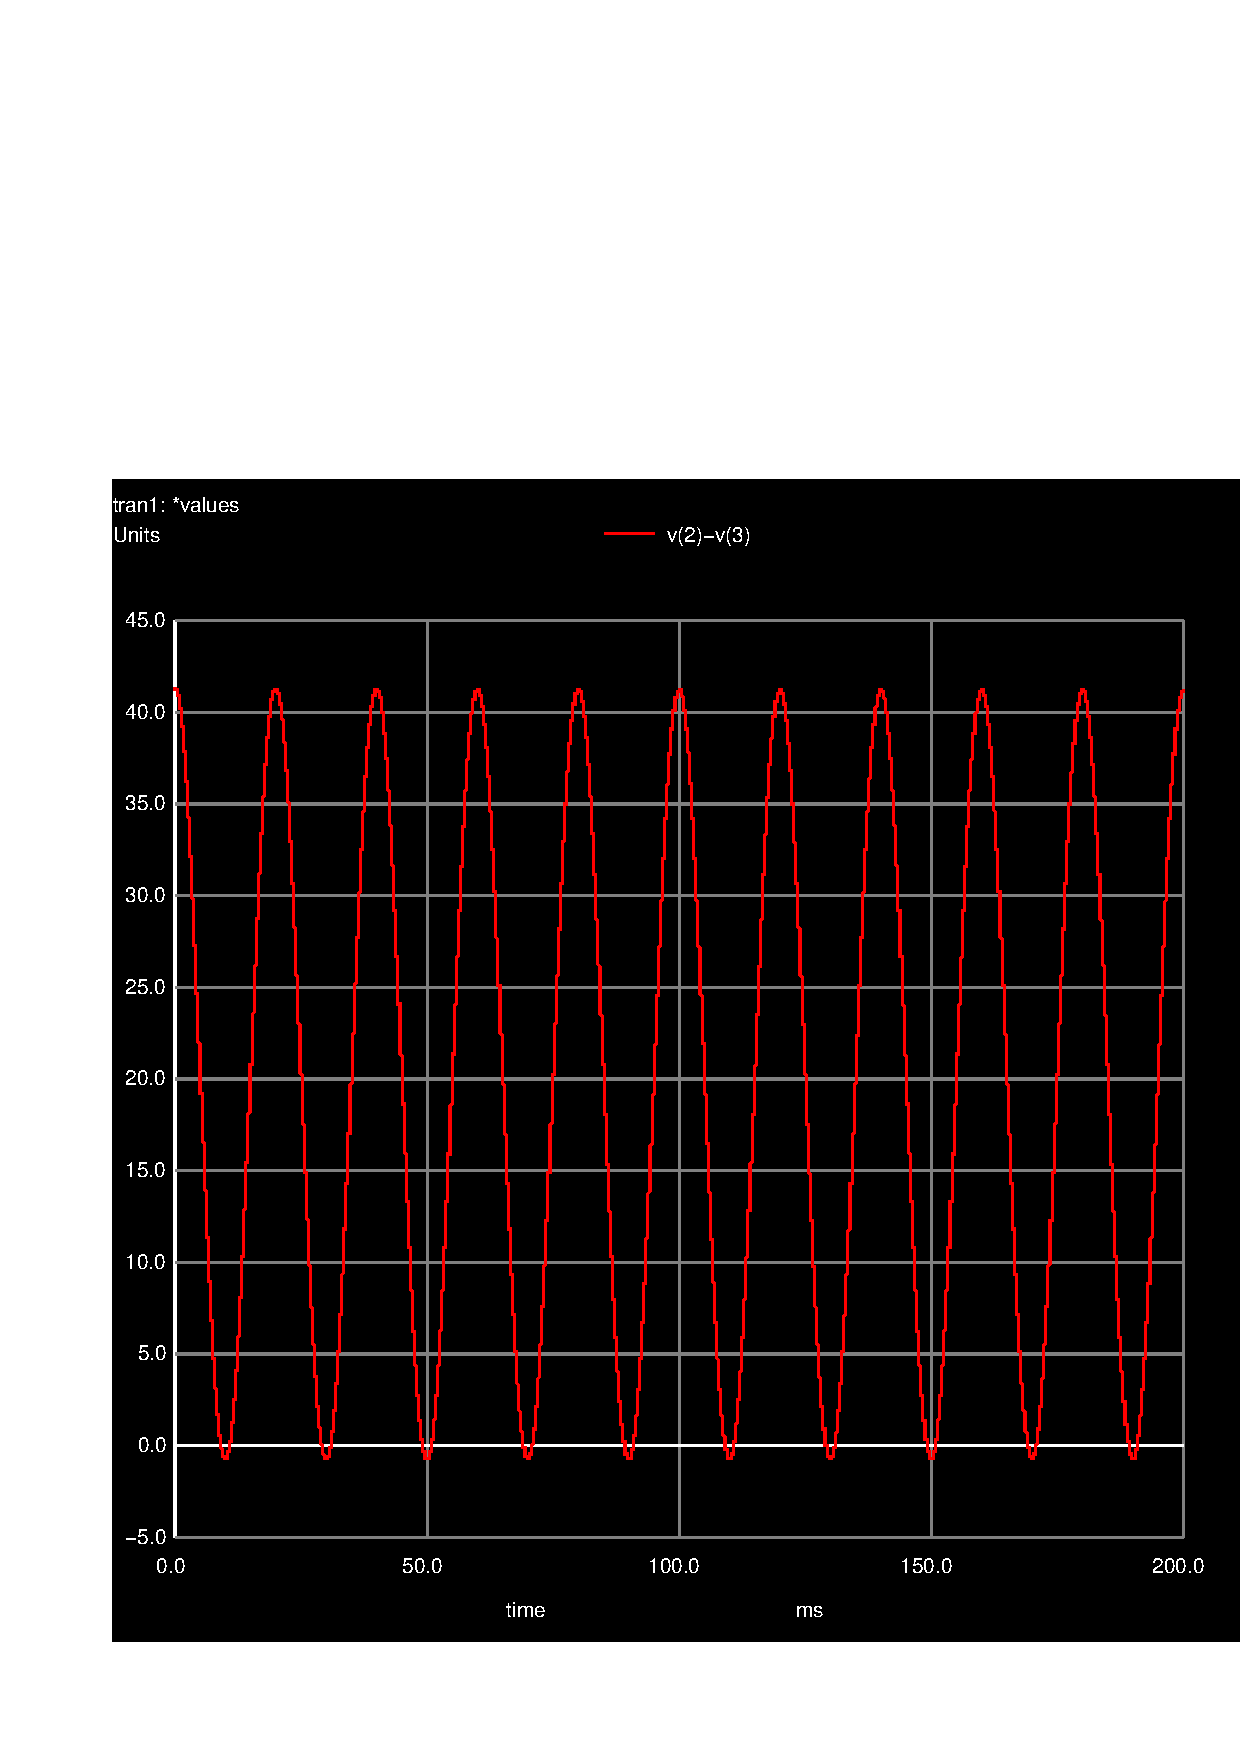
\includegraphics[width=0.6\linewidth]{vrect.pdf}
\caption{Output of the Envelope Detector (acting on the output of the full-wave rectifier)}
\label{fig:env}
\end{figure}

\subsection{Output of the voltage regulator circuit, compared with the input sinusoidal voltage and the envelope detector voltage}

\par
\begin{figure}[H] \centering
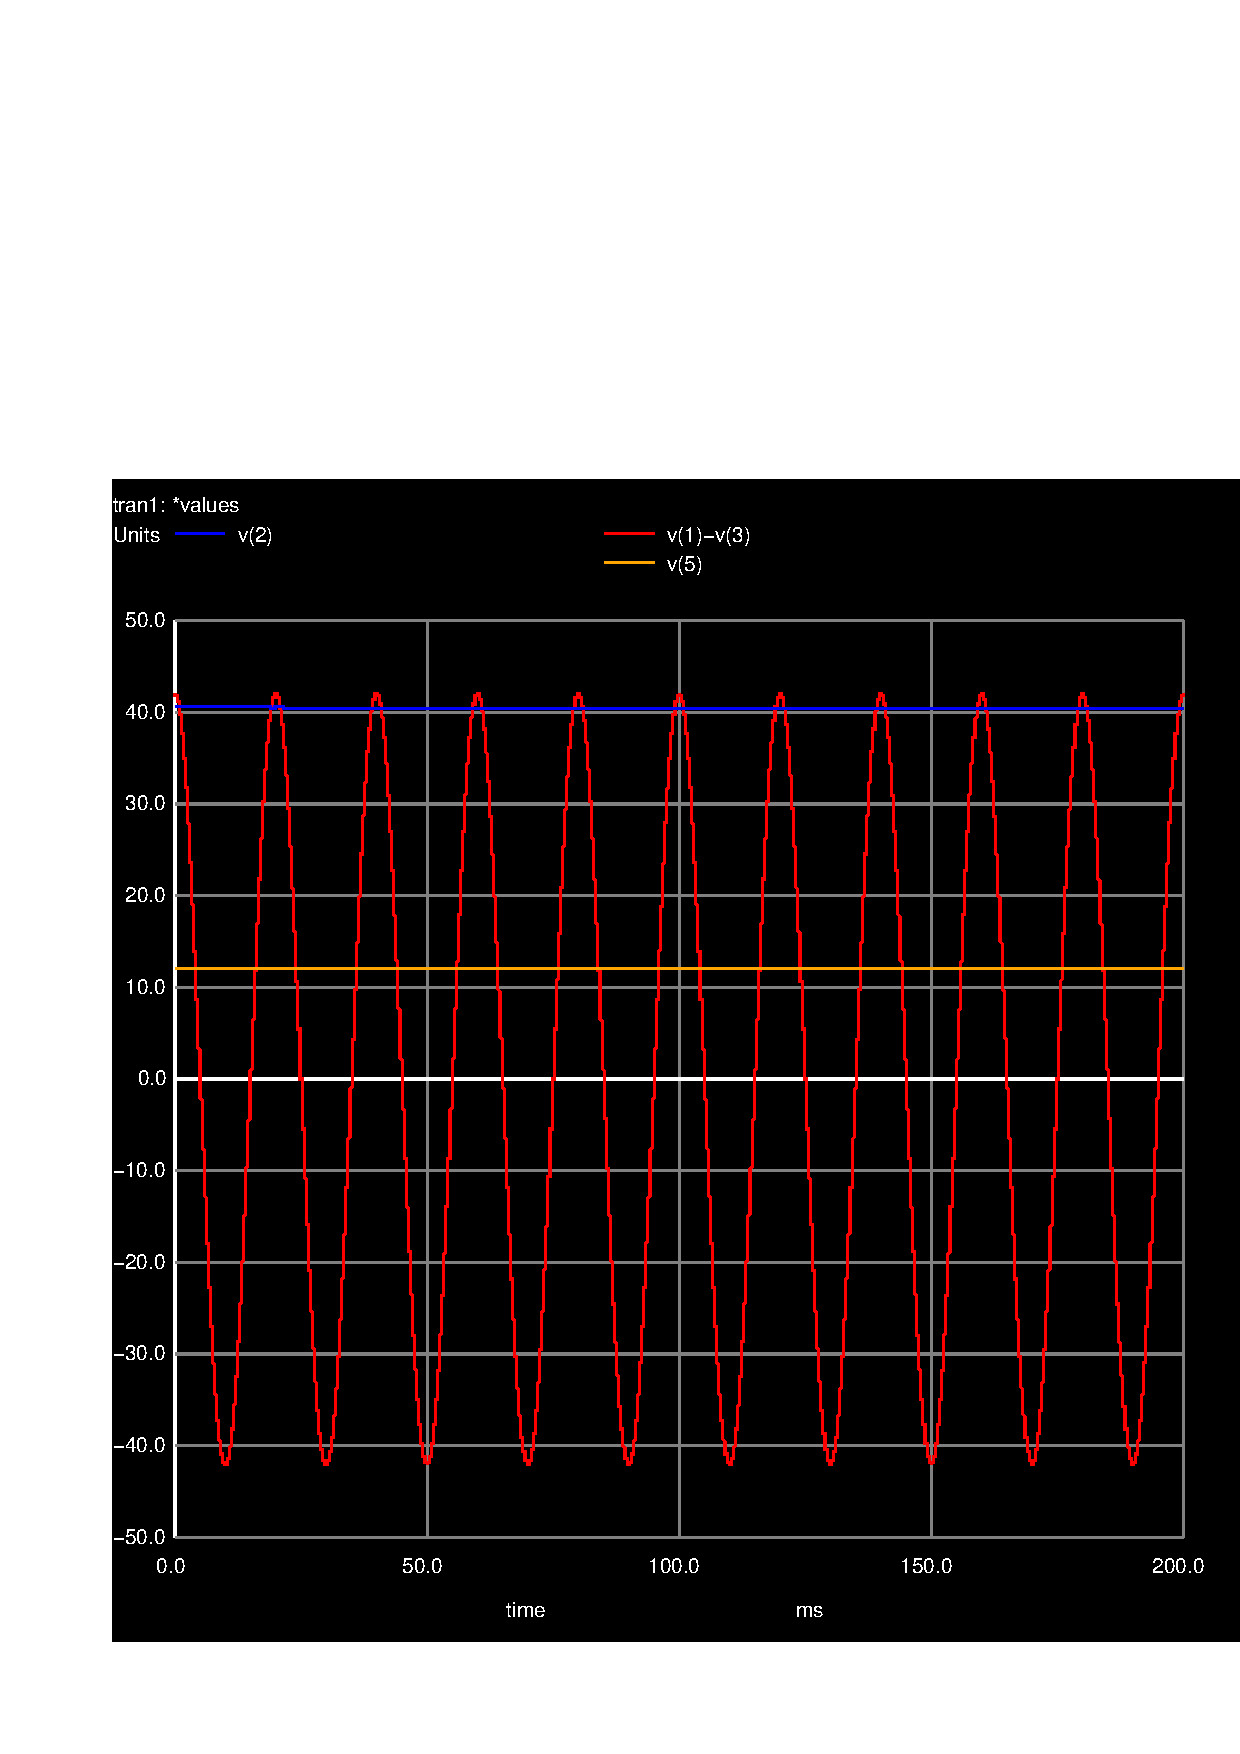
\includegraphics[width=0.6\linewidth]{vs_vout_venv.pdf}
\caption{Output of the voltage regulator circuit (yellow), compared with the input sinusoidal voltage (red) and the envelope detector voltage (blue)}
\label{fig:vs_venv_vout}
\end{figure}

\par
\begin{figure}[H] \centering
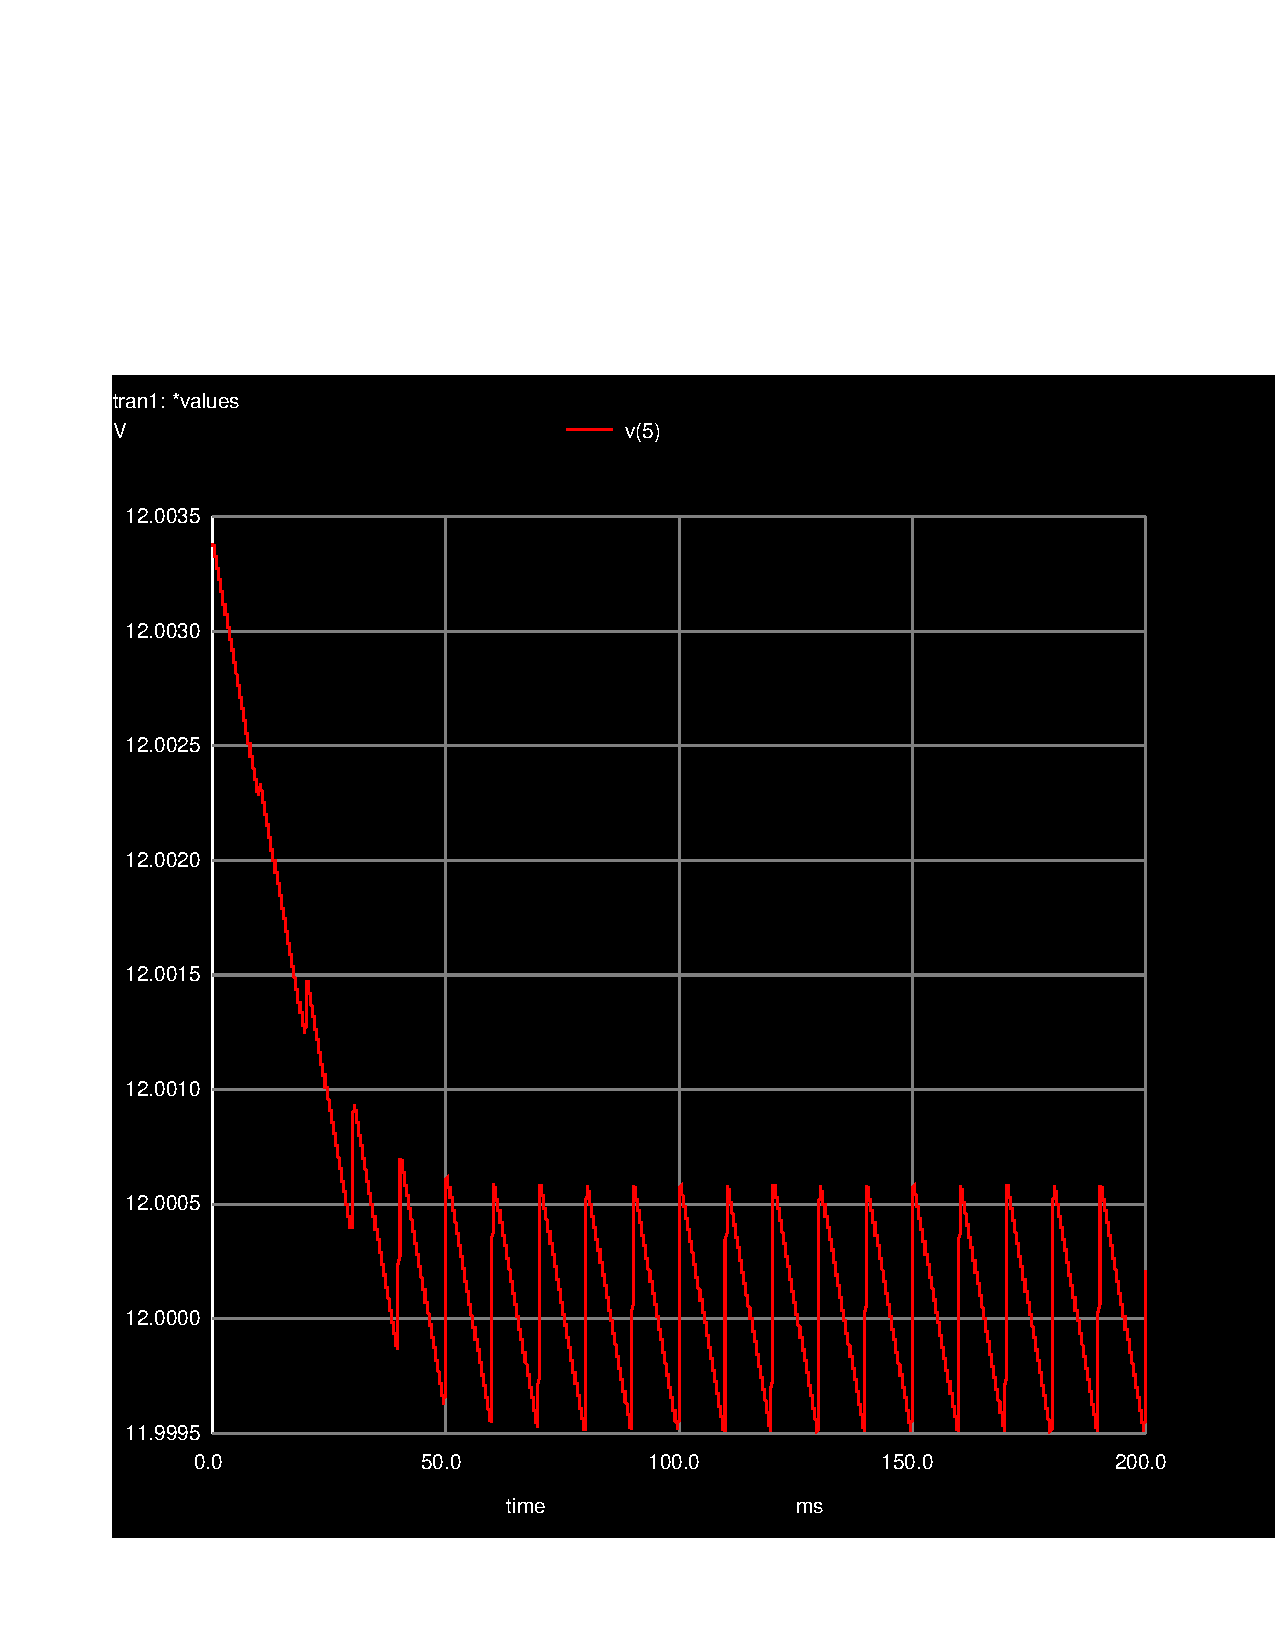
\includegraphics[width=0.6\linewidth]{vout.pdf}
\caption{Output of the voltage regulator circuit alone, so as to visualize the ripple effect in greater detail}
\label{fig:vout}
\end{figure}

\par
\begin{figure}[H] \centering
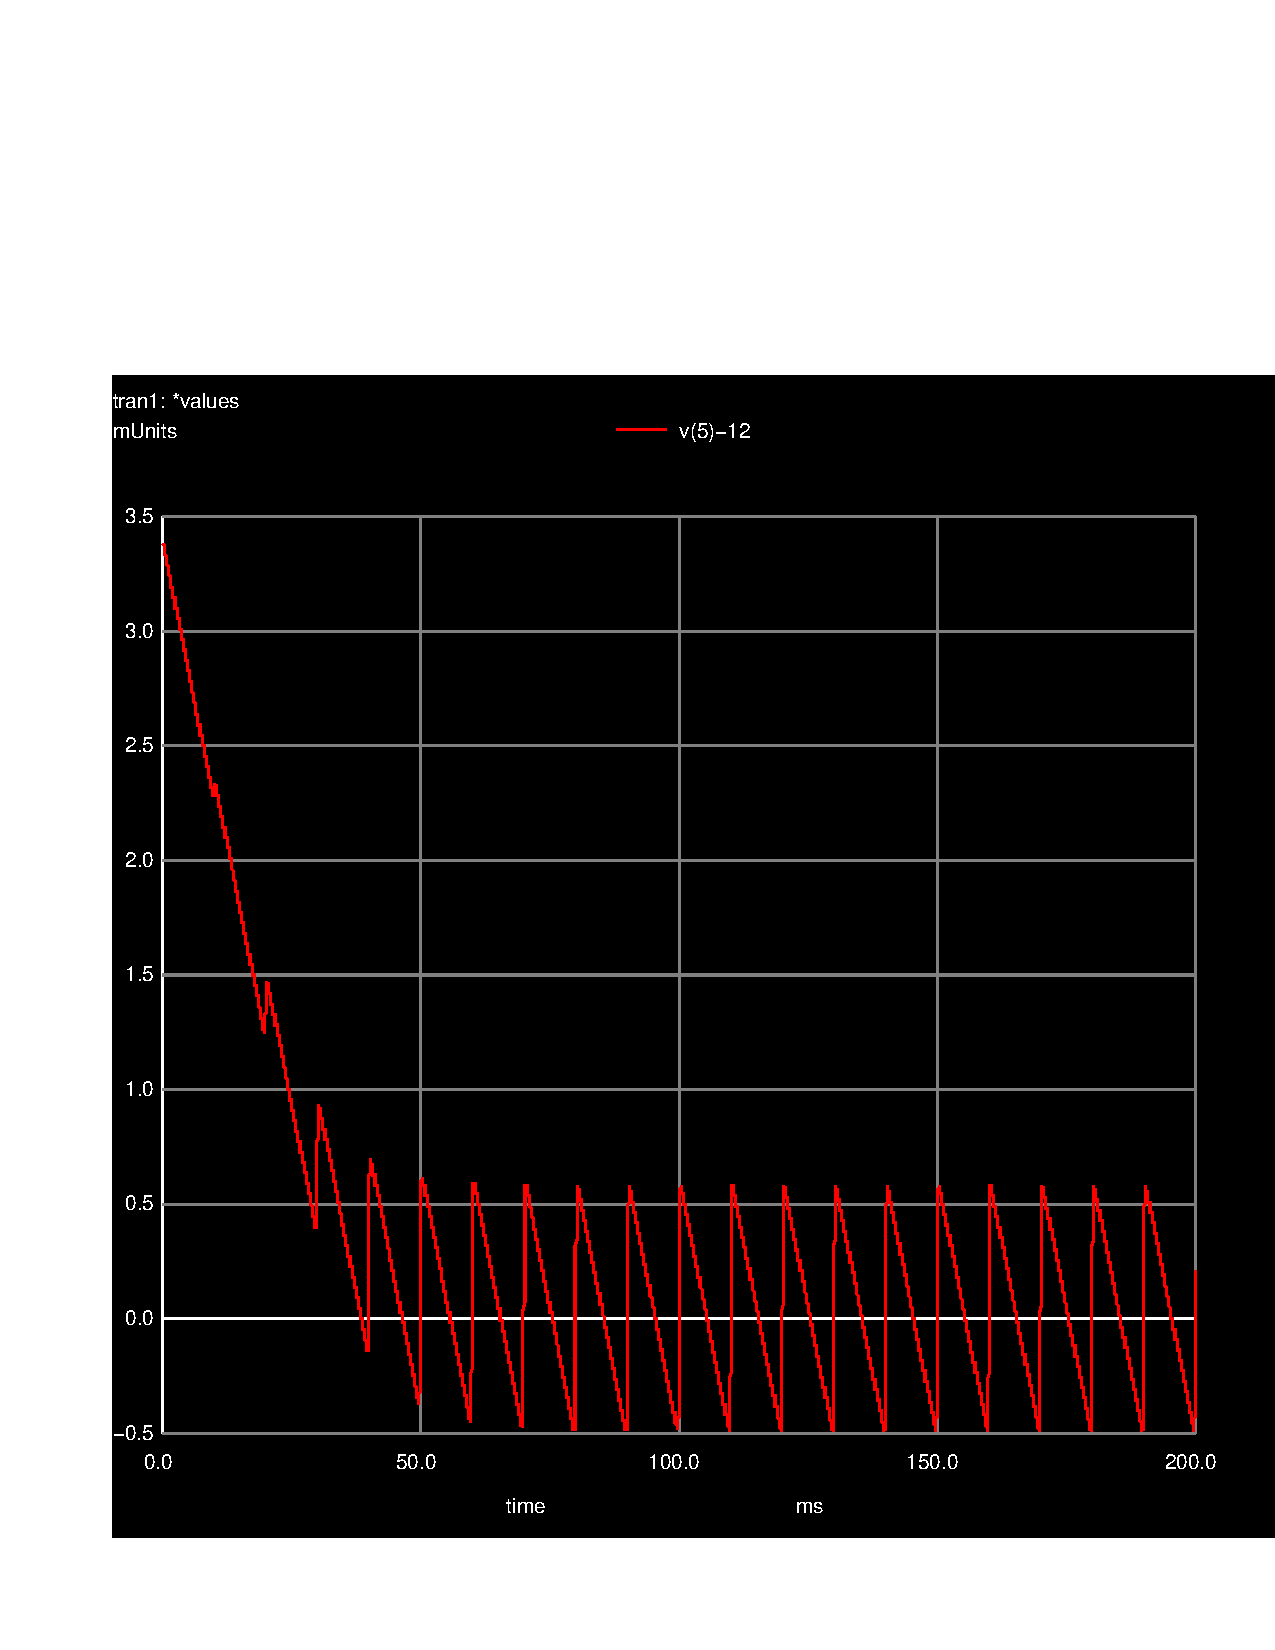
\includegraphics[width=0.6\linewidth]{vo_menos_12.pdf}
\caption{($v_O$ – 12) (output AC component + DC deviation) - note the vetical scale is in microVolts}
\label{fig:deviation}
\end{figure}

\pagebreak
